\documentclass[10pt]{beamer}
\usetheme{Malmoe}
\colorlet{beamer@blendedblue}{green!40!black}
\setbeamertemplate{navigation symbols}{}
\newcommand*\oldmacro{}%
\let\oldmacro\insertshorttitle%
\renewcommand*\insertshorttitle{%
\oldmacro\hfill%
\insertframenumber\,/\,\inserttotalframenumber}

\usepackage{caption}
\usepackage{hyperref}
\usepackage[makeroom]{cancel}
\usepackage{ amssymb }
\usepackage{appendixnumberbeamer}
%\usepackage{tikz-feynman}
\usepackage{graphicx}
\begin{document}
\title{Search for Flavor Changing Neutral Currents in Top Quark Decays}
\subtitle{$t \rightarrow q \gamma$}
\author[Barkeloo]{Jason Barkeloo}

\titlegraphic{
\includegraphics[width=4cm]{../ATLAS-Logo-Ref-RGB.png}\hspace*{2.75cm}~%
   
\includegraphics[width=4cm]{../uo_logo_green_on_white_2.jpg}
}

\date{January 18, 2018}
\frame{\titlepage}
%\frame{\frametitle{Table of Contents}\tableofcontents[hidesubsections]}
\section{Brief Background}
%\frame{\frametitle{Table of Contents}\tableofcontents[currentsection,hideothersubsections]}
%%%%%%%%%%%%%%%%%%%%%%%%%%%%%%%%%%%%%%%%%%%%%%%%%%%%%%%%%


\subsection{The Top Quark}

%%%%%%%%%%%%%%%%%%%%
\frame{\frametitle{The Top Quark}
\begin{itemize}
\item Heaviest fundamental particle, $172.5 GeV$
\item Lifetime $5x10^{-25}s$, decays before hadronization
	\begin{itemize}
	\item Allows us to study the decay of a single quark
	\end{itemize}
\end{itemize}
\begin{figure}
	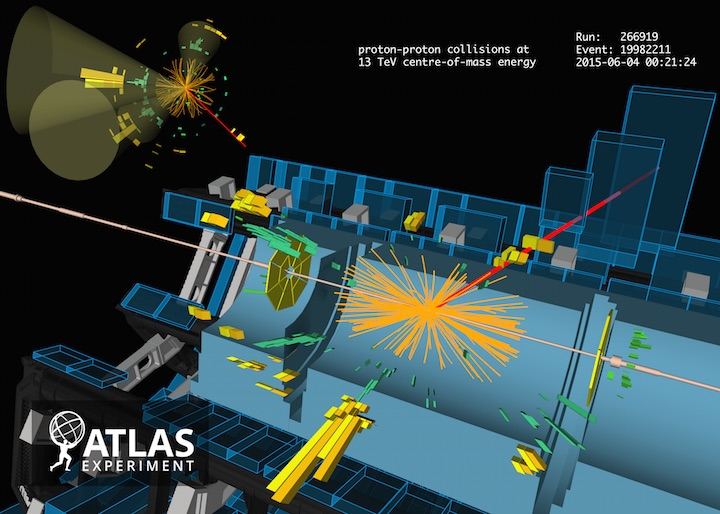
\includegraphics[height=0.5\textheight]{../../ThesisImages/ttbarevent.png}
	\captionof{figure}{$t\bar{t}$ event in the ATLAS detector}
\end{figure}
}

\frame{\frametitle{Top Quark Pair Production}
\begin{itemize}
\item Leading order processes for top quark production
	\begin{itemize}
	\item Quark-antiquark annihilation $\approx 10\%$
	\item Gluon-gluon fusion $\approx 90\%$
	\end{itemize}
\end{itemize}
\centering

	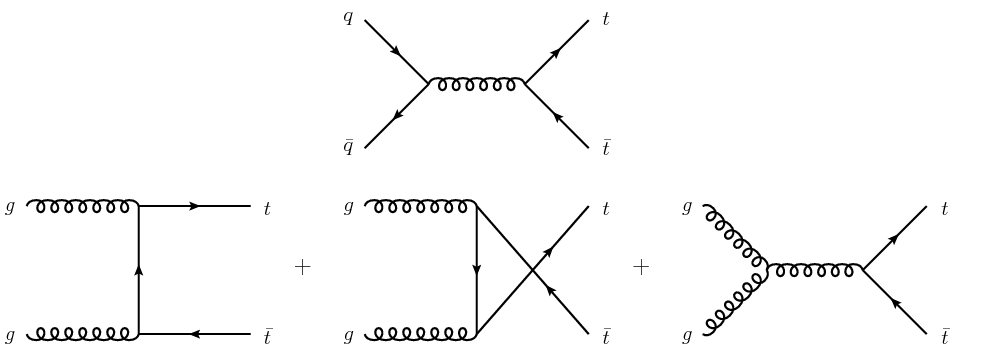
\includegraphics[height=0.5\textheight]{../../ThesisImages/LOPairProdDiags.png}
	\captionof{figure}{Leading order $t\bar{t}$ diagrams}
}

\frame{\frametitle{Top Quark Pair Production}
\begin{itemize}
\item At $\sqrt{s}=13TeV$ for $m_{t}=172.5GeV$, $\sigma_{t\bar{t}} = 831.76pb$
\end{itemize}
\centering
	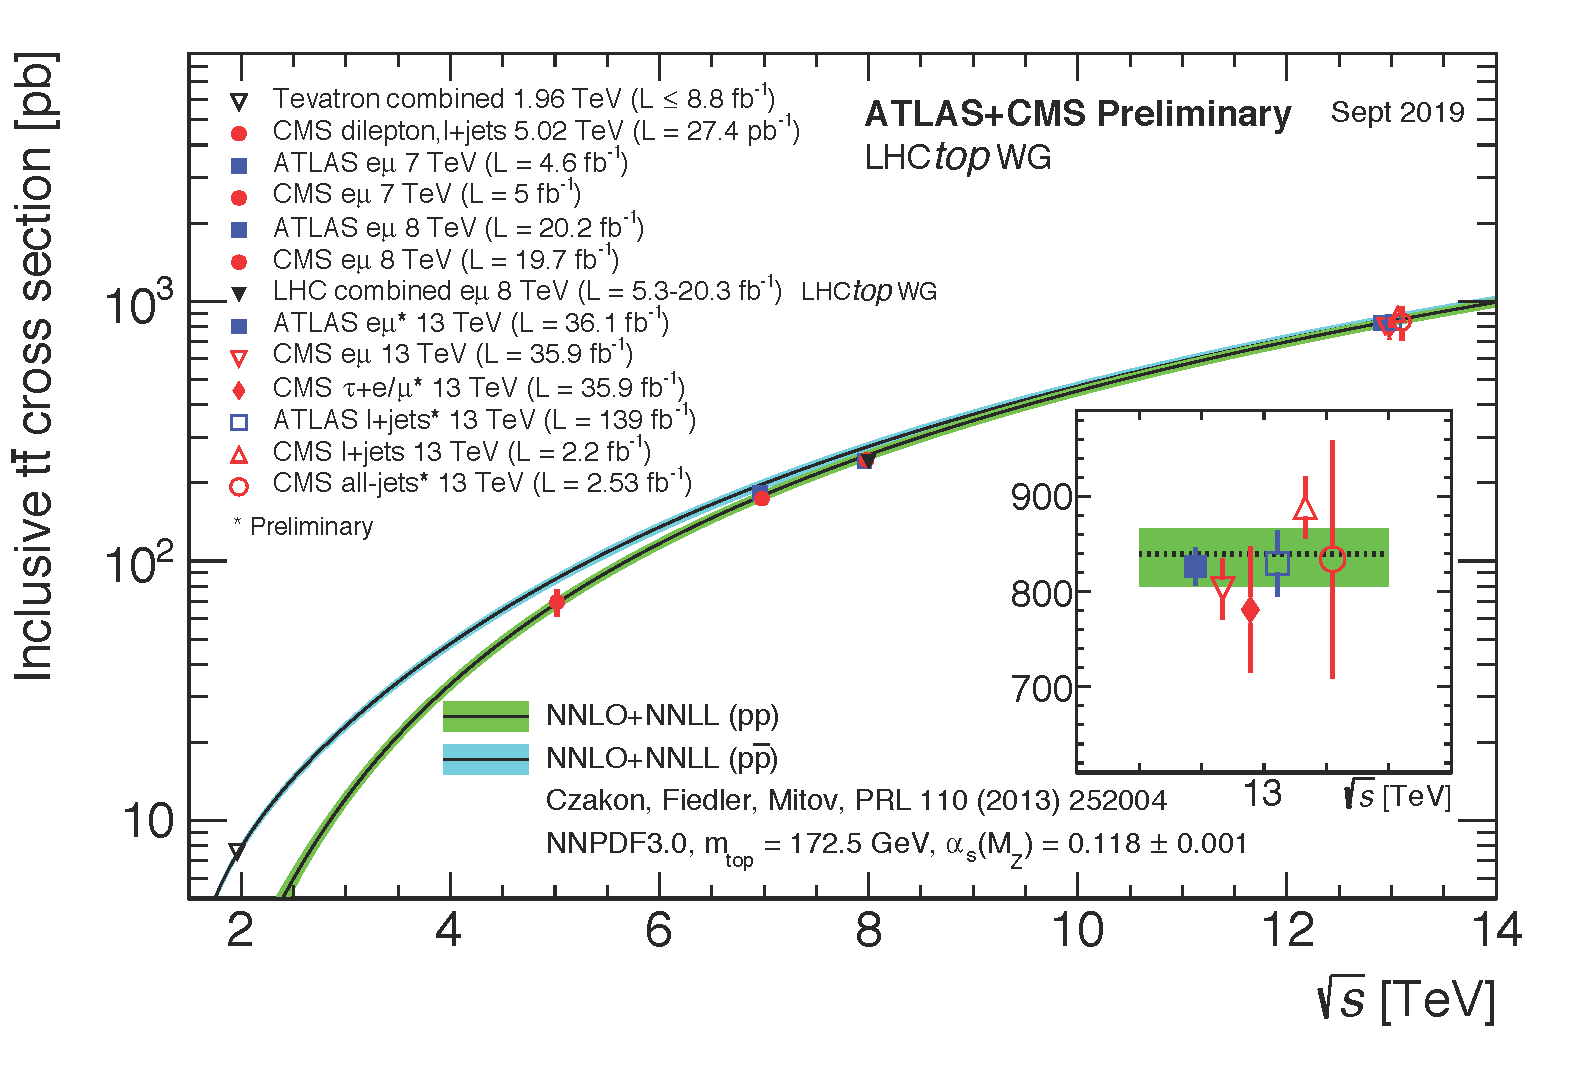
\includegraphics[height=0.7\textheight]{../../ThesisImages/ttprodxsec.png}
	\captionof{figure}{$t\bar{t}$ production cross section \href{https://twiki.cern.ch/twiki/bin/view/LHCPhysics/LHCTopWGSummaryPlots}{[TopWGSummaryPlots]}}
}

\frame{\frametitle{Top Quark Decays}
\begin{columns}
\begin{column}{0.5\textwidth}
\begin{itemize}
\item Standard model top branching ratio to bW $\simeq 100\%$
\end{itemize}
\centering
 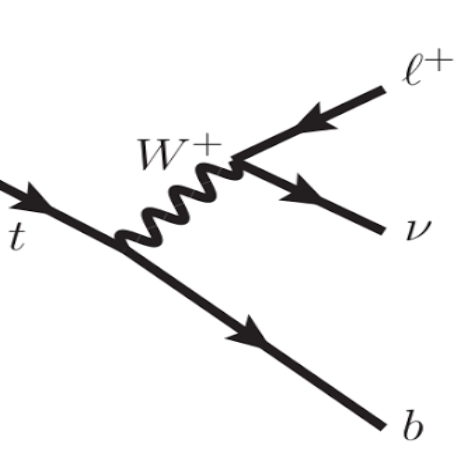
\includegraphics[width=0.7\textwidth]{../../ThesisImages/topdecay.png}
 \captionof{figure}{Leptonic final state diagram for a top decay}
\end{column}
\begin{column}{0.5\textwidth}  %%<--- here
     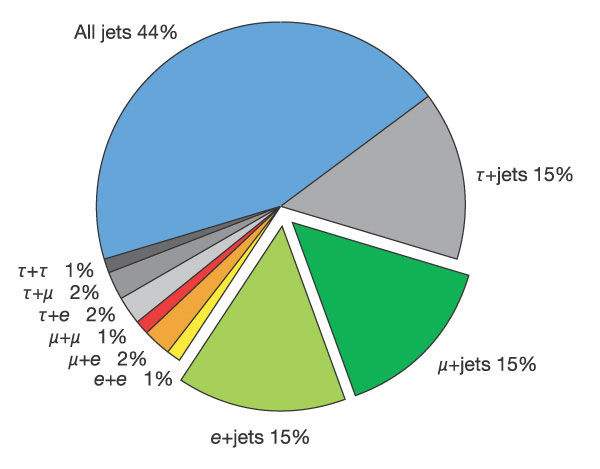
\includegraphics[width=1.1\textwidth]{../../ThesisImages/topdecayproducts.jpg}
    \captionof{figure}{Top quark pair decay final states \href{https://images.nature.com/full/nature-assets/nature/journal/v429/n6992/images/nature02589-f2.2.jpg}{[Nature]}}
\end{column}
\end{columns}
}

\frame{\frametitle{Top Quark Decays in the SM}
\centering
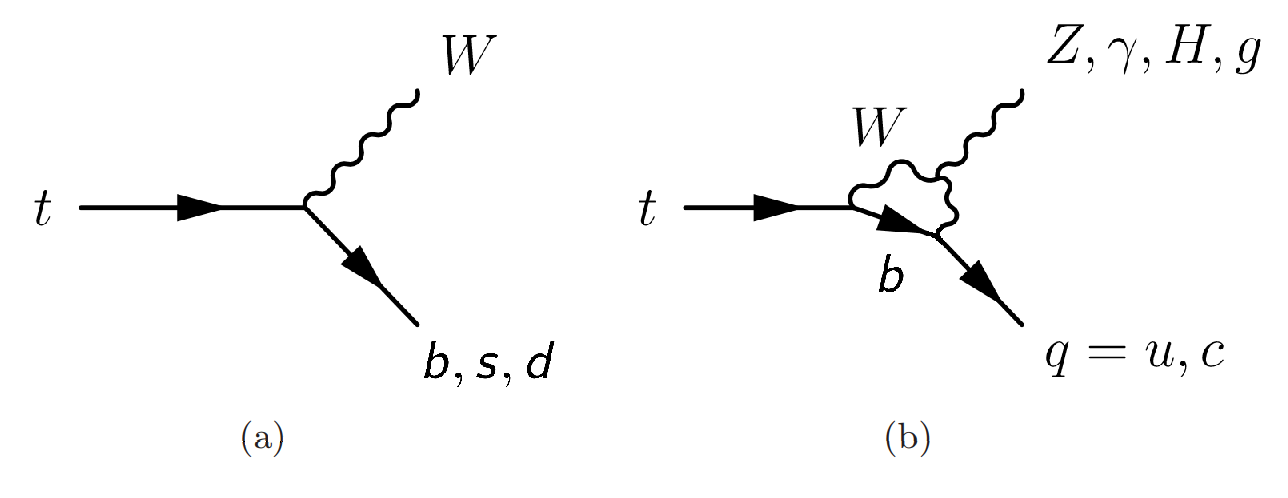
\includegraphics[width=1.\textwidth]{../../ThesisImages/SMTopDecays.png}

\begin{columns}
\begin{column}{0.5\textwidth}
\begin{itemize}
\item $t\rightarrow b W \approx 99.83\%$
\item $t\rightarrow s W \approx 0.16\%$
\item $t\rightarrow d W \approx 0.01\%$
\end{itemize}
\end{column}
\begin{column}{0.5\textwidth}
\begin{itemize}
\item $t\rightarrow q_{u,c} X\approx 10^{-17} - 10^{-12}$
\end{itemize}
\end{column}
\end{columns}

%\feynmandiagram [small,horizontal=a to b] {
%  a [particle=\(t\)] -- [fermion] b ,
% f1 [particle=\({b,s,d} \)] -- b -- [boson] f2 [ particle=\(W\)],
%};
}





\subsection{FCNC at the LHC}
\frame{\frametitle{FCNC: What are we looking for? $t\bar{t}\rightarrow W (\rightarrow l \nu) b+ q\gamma$}
\begin{itemize}
\item Final state topology
	\begin{itemize}
	\item One Neutrino, from W
	\item One Lepton, from W
	\item One B-jet, SM top
	\item One Photon, FCNC Top
	\item One Jet, FCNC Top
	\end{itemize}
\end{itemize}
\centering
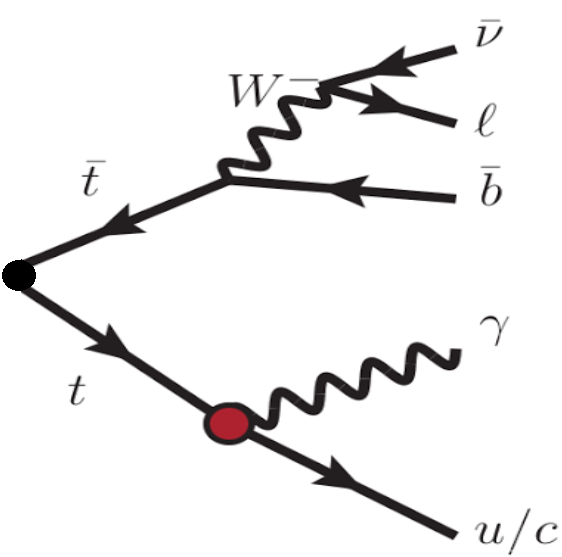
\includegraphics[width=0.4\textwidth]{../../ThesisImages/fcncttbar.png}
}

\frame{\frametitle{Background Processes}
\begin{itemize}
\item Due to all of the processes at hadron colliders it is important to model similar event topologies well.
\item Major backgrounds include $t\bar{t}$, W+Jets, Z+Jets, + processes with an associated photon
\end{itemize}
\centering
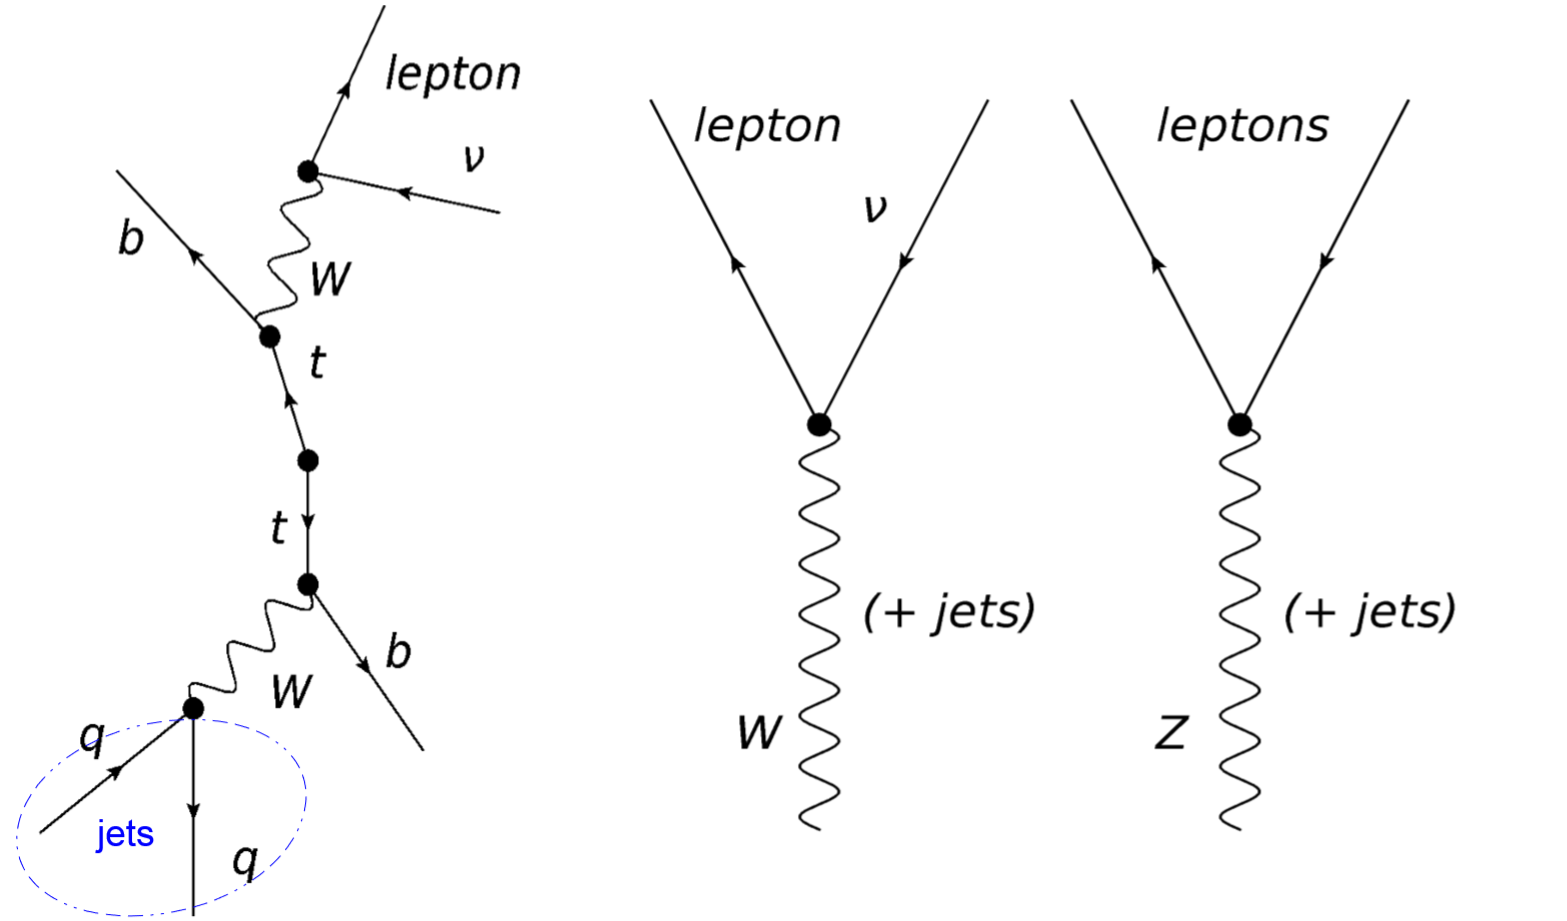
\includegraphics[width=0.7\textwidth]{../../ThesisImages/backgrounds.png}
}


%%%%%%%%%%%%%%%%%%%%%%%%%%%%%%%%%%%%%%%%%%%%%%%%%%%%%%%%%%%%%%%%%
\section{Searching for Flavor Changing Neutral Current Signatures}

\subsection{FCNCs with Photons}

\subsection{Object Preselection Cuts}


\frame{\frametitle{Object Preselection}
\begin{itemize}
\item We preselect events with objects that look like our expected topology
\item Require:
	\begin{itemize}
	\item Exactly one lepton (e or $\mu$) $\geq$ 28 GeV
	\item Exactly one Good photon $\geq$ 25GeV
	\item Missing Transverse Energy $\geq$ 30GeV
	\item $\geq 2$ Jets (at least one being b-tagged)
	\end{itemize}
\item All following plots will have signal scaled to $1\%$ of $\sigma_{t\bar{t}}$, MC scaled to $36.07fb^{-1}$
\end{itemize}
}


\frame{\frametitle{Preselection Objects}

\begin{columns}
\begin{column}{0.02\textwidth}

\rotatebox{90}{Muon Channel \qquad  Electron Channel} 
%\rotatebox{90}{Muon Channel        } 
\end{column}
\begin{column}{0.33\textwidth}
\begin{itemize}
\item  Leading Jet $p_T$
\end{itemize}
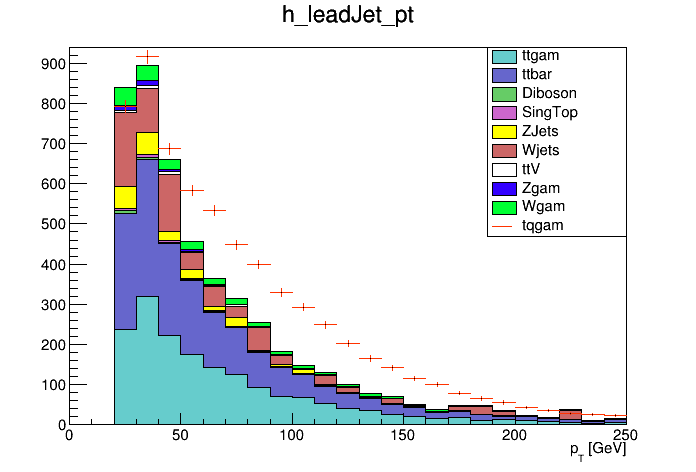
\includegraphics[width=1.1\textwidth]{../../ThesisImages/plotsloose/el_h_leadJet_pt.png} \\
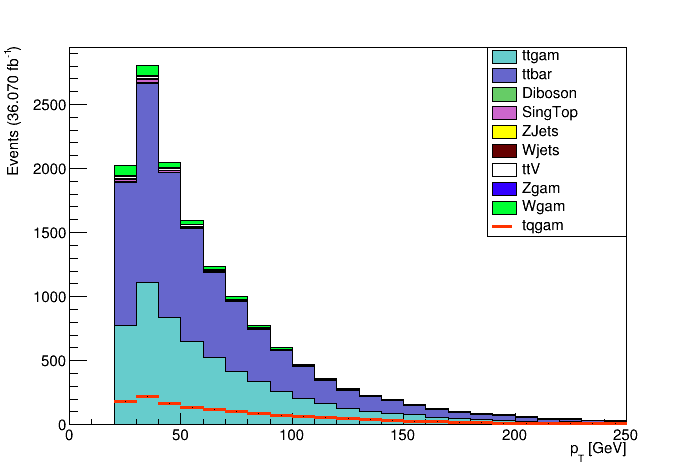
\includegraphics[width=1.1\textwidth]{../../ThesisImages/plotsloose/mu_h_leadJet_pt.png}
\end{column}
\begin{column}{0.33\textwidth}
\begin{itemize}
\item Photons
\end{itemize}
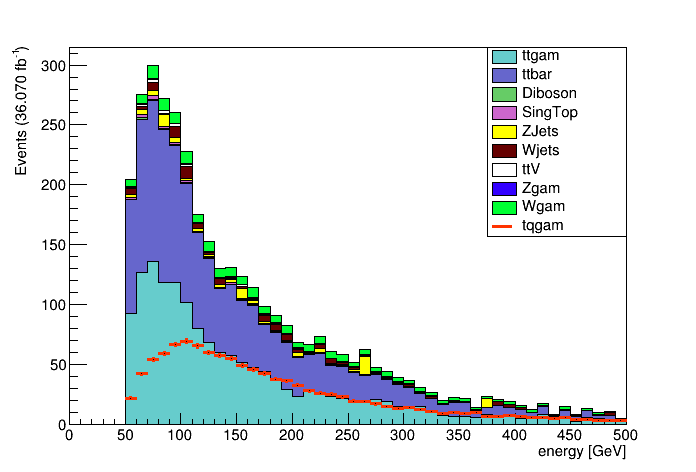
\includegraphics[width=1.1\textwidth]{../../ThesisImages/plotsloose/el_h_photon_e.png} \\
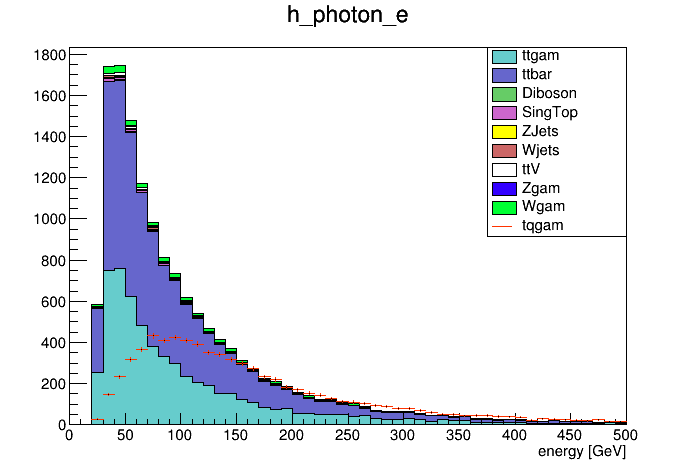
\includegraphics[width=1.1\textwidth]{../../ThesisImages/plotsloose/mu_h_photon_e.png}
\end{column}
\begin{column}{0.33\textwidth}
\begin{itemize}
\item Leptons
\end{itemize}
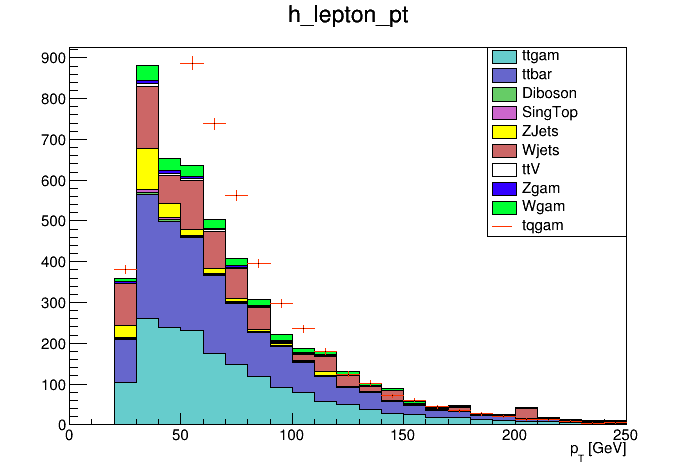
\includegraphics[width=1.1\textwidth]{../../ThesisImages/plotsloose/el_h_lepton_pt.png}\\
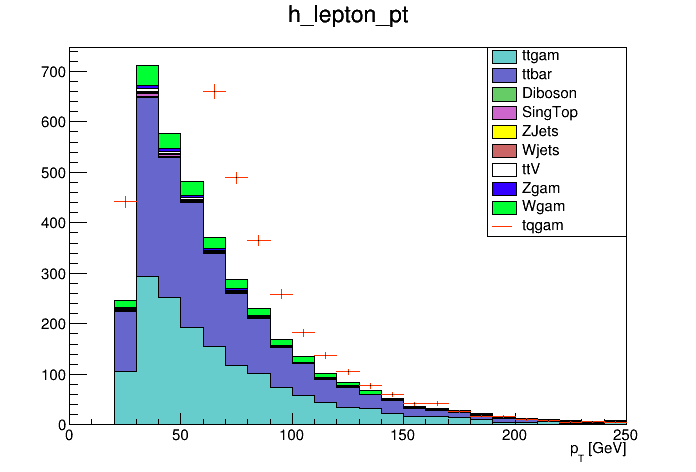
\includegraphics[width=1.1\textwidth]{../../ThesisImages/plotsloose/mu_h_lepton_pt.png}
\end{column}
\end{columns}
}


\subsection{Top and Neutrino Reconstruction}
\frame{\frametitle{Where are the Tops?}
\begin{itemize}
\item Must be 'reconstructed' from these objects as well as b-jets and $E_T^{miss}$
\item $E_T^{miss}$ is calculated to balance the event energy in the transverse plane of the detector
\item The other particles are combined in the only way the signal topology would allow two top quark candidates
\begin{itemize}
\item Standard model top candidate: b-jet + lepton + neutrino 
\item FCNC Top: Photon + Light Jet
\end{itemize}
\end{itemize}
}

%%%%%%%%%%%%%%%%


\frame{\frametitle{Neutrinos}
\begin{itemize}
\item All missing energy in signal topology is from neutrino
\item We have $E_T^{miss}$ and its' direction   
\begin{itemize}
\item Can calulate  $E_{Tx}^{miss}$ and  $E_{Ty}^{miss}$ easily
\item Ambiguous direction along the z-axis
\end{itemize}
\item A minimization of this $\chi^2$ will allow us to determine the z momentum of the neutrino: $\chi^2 = \frac{(m_{b,l,\nu}-m_t)^2}{\sigma^2_{SMtop}}+\frac{(m_{l,\nu}-m_W)^2}{\sigma^2_W} $
\end{itemize}

%\[ \chi^2 = \frac{(m_{b,l,\nu}-m_t)^2}{\sigma^2_{SMtop}}+\frac{(m_{l,\nu}-m_W)^2}{\sigma^2_W}  \]
\begin{columns}
\begin{column}{0.5\textwidth}
\centering
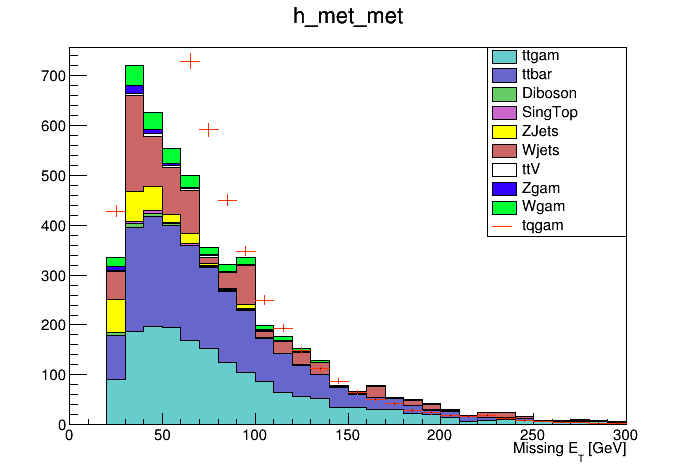
\includegraphics[width=.9\textwidth]{../../ThesisImages/plotsloose/el_h_met_met.png}
\captionof{figure}{e-channel $E_T^{miss}$ distribution}
\end{column} 
\begin{column}{0.5\textwidth}
\centering
\includegraphics[width=.9\textwidth]{../../ThesisImages/plotsloose/el_h_min_chi2.png}
\captionof{figure}{e-channel $\chi^2$ distribution}
\end{column}
\end{columns}
}

\frame{\frametitle{Reconstructed Tops}
\begin{columns}
\begin{column}{0.02\textwidth}
\rotatebox{90}{Muon Channel \qquad  Electron Channel} 
\end{column}
\begin{column}{0.5\textwidth}
\begin{itemize}
\item SM Top
\end{itemize}
\centering
\includegraphics[width=.9\textwidth]{../../ThesisImages/plotsloose/el_h_sm_top_m.png}\\
\includegraphics[width=.9\textwidth]{../../ThesisImages/plotsloose/mu_h_sm_top_m.png}
\end{column} 
\begin{column}{0.5\textwidth}
\begin{itemize}
\item FCNC Top
\end{itemize}
\centering
\includegraphics[width=.9\textwidth]{../../ThesisImages/plotsloose/el_h_qgam_m.png}\\
\includegraphics[width=.9\textwidth]{../../ThesisImages/plotsloose/mu_h_qgam_m.png}
\end{column}
\end{columns}
}


\frame{\frametitle{Thinning Out Backgrounds}
\begin{columns}
\begin{column}{0.02\textwidth}
\rotatebox{90}{Muon Channel \qquad  Electron Channel} 
\end{column}
\begin{column}{0.5\textwidth}
\begin{itemize}
\item Reconstructing Z mass
\end{itemize}
\centering
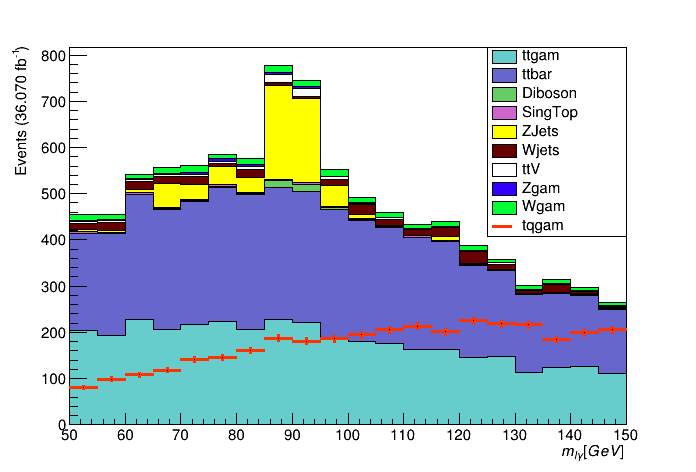
\includegraphics[width=.9\textwidth]{../../ThesisImages/plotsloose/el_h_lgam_m.png}\\
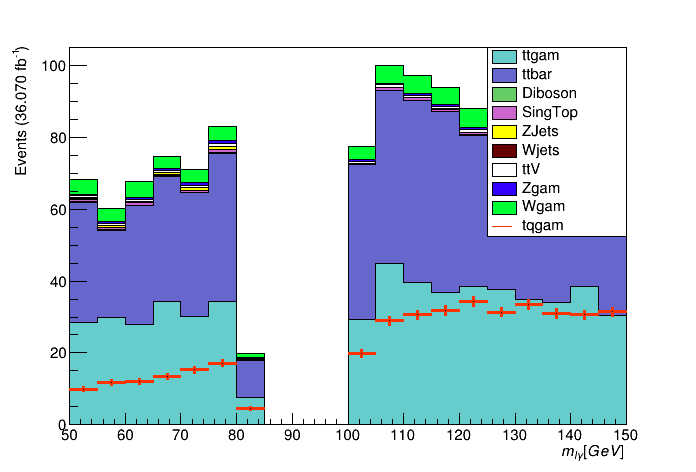
\includegraphics[width=.9\textwidth]{../../ThesisImages/plotsloose/mu_h_lgam_m.png}
\end{column} 
\begin{column}{0.5\textwidth}
\begin{itemize}
\item Number of BJets
\end{itemize}
\centering
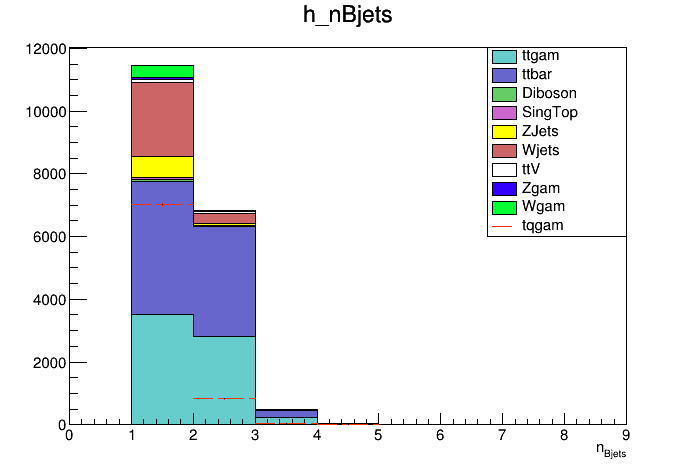
\includegraphics[width=.9\textwidth]{../../ThesisImages/plotsloose/el_h_nBjets.png}\\
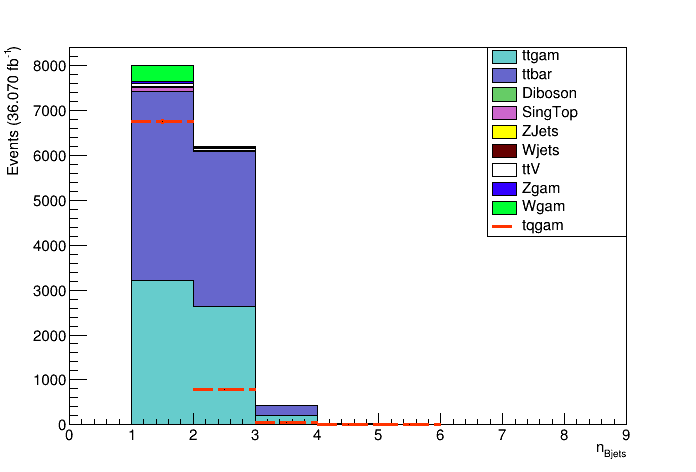
\includegraphics[width=.9\textwidth]{../../ThesisImages/plotsloose/mu_h_nBjets.png}
\end{column}
\end{columns}
}

\frame{\frametitle{Thinning Out Backgrounds: SM Top ($m_{l \nu b}$)}
\begin{columns}
\begin{column}{0.02\textwidth}
\rotatebox{90}{Muon Channel \qquad  Electron Channel} 
\end{column}
\begin{column}{0.5\textwidth}
\begin{itemize}
\item Before Z-mass, Bjet cuts
\end{itemize}
\centering
\includegraphics[width=.9\textwidth]{../../ThesisImages/plotsloose/el_h_sm_top_m.png}\\
\includegraphics[width=.9\textwidth]{../../ThesisImages/plotsloose/mu_h_sm_top_m.png}
\end{column} 
\begin{column}{0.5\textwidth}
\begin{itemize}
\item After Cuts
\end{itemize}
\centering
\includegraphics[width=.9\textwidth]{../../ThesisImages/plotsstrict/el_h_sm_top_m.png}\\
\includegraphics[width=.9\textwidth]{../../ThesisImages/plotsstrict/mu_h_sm_top_m.png}
\end{column}
\end{columns}
}

\frame{\frametitle{Thinning Out Backgrounds: FCNC Top ($m_{q \gamma}$)}
\begin{columns}
\begin{column}{0.02\textwidth}
\rotatebox{90}{Muon Channel \qquad  Electron Channel} 
\end{column}
\begin{column}{0.5\textwidth}
\begin{itemize}
\item Before Z-mass, Bjet cuts
\end{itemize}
\centering
\includegraphics[width=.9\textwidth]{../../ThesisImages/plotsloose/el_h_qgam_m.png}\\
\includegraphics[width=.9\textwidth]{../../ThesisImages/plotsloose/mu_h_qgam_m.png}
\end{column} 
\begin{column}{0.5\textwidth}
\begin{itemize}
\item After Cuts
\end{itemize}
\centering
\includegraphics[width=.9\textwidth]{../../ThesisImages/plotsstrict/el_h_qgam_m.png}\\
\includegraphics[width=.9\textwidth]{../../ThesisImages/plotsstrict/mu_h_qgam_m.png}
\end{column}
\end{columns}
}

\section{Current Investigations}
\subsection{$\chi^2$}
\frame{\frametitle{Current Investigation: $\chi^2$ }
\begin{itemize}
\item Can $\chi^2$ be used as a discriminating variable?

\item  $\chi^2 = \frac{(m_{b,l,\nu}-m_t)^2}{\sigma^2_{SMtop}}+\frac{(m_{l,\nu}-m_W)^2}{\sigma^2_W} $
\end{itemize}

\begin{columns}
\begin{column}{0.5\textwidth}
\centering
\includegraphics[width=.9\textwidth]{../../ThesisImages/plotsloose/el_h_min_chi2.png}
\captionof{figure}{e-channel $\chi^2$ before cuts}
\end{column} 
\begin{column}{0.5\textwidth}
\centering
\includegraphics[width=.9\textwidth]{../../ThesisImages/plotsstrict/el_h_min_chi2.png}
\captionof{figure}{e-channel $\chi^2$ after Z, Bjet cuts}
\end{column}
\end{columns}
}

\frame{\frametitle{Current Investigation: $\chi^2$ }

\begin{columns}
\begin{column}{0.02\textwidth}
\rotatebox{90}{After Cuts \qquad \qquad  Before Cuts} 
\end{column}
\begin{column}{0.5\textwidth}
\begin{itemize}
\item  $\frac{(m_{b,l,\nu}-m_t)^2}{\sigma^2_{SMtop}}$
\end{itemize}
\centering
\includegraphics[width=.9\textwidth]{../../ThesisImages/plotsloose/mu_h_w_chi2.png}\\
\includegraphics[width=.9\textwidth]{../../ThesisImages/plotsstrict/mu_h_w_chi2.png}
\end{column} 
\begin{column}{0.5\textwidth}
\begin{itemize}
\item $ \frac{(m_{l,\nu}-m_W)^2}{\sigma^2_W}$
\end{itemize}
\centering
\includegraphics[width=.9\textwidth]{../../ThesisImages/plotsloose/mu_h_sm_chi2.png}\\
\includegraphics[width=.9\textwidth]{../../ThesisImages/plotsstrict/mu_h_sm_chi2.png}
\end{column}
\end{columns}


}

\subsection{Photon Isolation}
\frame{\frametitle{Current Investigation: Photon Isolation: $\mu$-Channel}

\begin{columns}
\begin{column}{0.02\textwidth}

\rotatebox{90}{After Cuts \qquad \qquad  Before Cuts} 
%\rotatebox{90}{Muon Channel        } 
\end{column}
\begin{column}{0.33\textwidth}
\begin{itemize}
\item ptvarcone20
\end{itemize}
\includegraphics[width=1.1\textwidth]{../../ThesisImages/plotsloose/mu_h_ph_ptvarcone20.png} \\
\includegraphics[width=1.1\textwidth]{../../ThesisImages/plotsstrict/mu_h_ph_ptvarcone20.png}
\end{column}
\begin{column}{0.33\textwidth}
\begin{itemize}
\item ptvarcone30
\end{itemize}
\includegraphics[width=1.1\textwidth]{../../ThesisImages/plotsloose/mu_h_ph_ptvarcone30.png} \\
\includegraphics[width=1.1\textwidth]{../../ThesisImages/plotsstrict/mu_h_ph_ptvarcone30.png}
\end{column}
\begin{column}{0.33\textwidth}
\begin{itemize}
\item topoetcone20
\end{itemize}
\includegraphics[width=1.1\textwidth]{../../ThesisImages/plotsloose/mu_h_ph_topoetcone20.png} \\
\includegraphics[width=1.1\textwidth]{../../ThesisImages/plotsstrict/mu_h_ph_topoetcone20.png}
\end{column}
\end{columns}
}

\subsection{Geometric Considerations}
\frame{\frametitle{Current Investigation: Geometry $\Delta$R to $\gamma$: e-channel}

\begin{columns}
\begin{column}{0.02\textwidth}

\rotatebox{90}{After Cuts \qquad \qquad  Before Cutsl} 
%\rotatebox{90}{Muon Channel        } 
\end{column}
\begin{column}{0.33\textwidth}
\begin{itemize}
\item $\Delta R_{\gamma l}$
\end{itemize}
\includegraphics[width=1.1\textwidth]{../../ThesisImages/plotsloose/el_h_ph_drlept.png} \\
\includegraphics[width=1.1\textwidth]{../../ThesisImages/plotsstrict/el_h_ph_drlept.png}
\end{column}
\begin{column}{0.33\textwidth}
\begin{itemize}
\item $\Delta R_{\gamma j_0}$
\end{itemize}
\includegraphics[width=1.1\textwidth]{../../ThesisImages/plotsloose/el_h_ph_drleadjet.png} \\
\includegraphics[width=1.1\textwidth]{../../ThesisImages/plotsstrict/el_h_ph_drleadjet.png}
\end{column}
\begin{column}{0.33\textwidth}
\begin{itemize}
\item $\Delta R_{\gamma j_1}$
\end{itemize}
\includegraphics[width=1.1\textwidth]{../../ThesisImages/plotsloose/el_h_ph_drsubljet.png} \\
\includegraphics[width=1.1\textwidth]{../../ThesisImages/plotsstrict/el_h_ph_drsubljet.png}
\end{column}
\end{columns}
}

%%%%%%%%%%%%%%%%%%%%%%%%%%%%%%%%%%%%%%%%%%%%%%%%%%%%%%%%%%%%%%%%%%
\section{}
\subsection{Outlook}
\frame{\frametitle{Outlook}
\begin{itemize}
\item Many improvements can be made to the analysis
\begin{itemize}
\item Further investigation of $\chi^2$ cuts 
\item Inclusion of a new term in $\chi^2$ to do with FC
\item Isolation cuts don't seem too promising for background reduction
\item $\Delta R_{\gamma l}$ could be useful
\end{itemize}
\item Monte Carlo distributions can be used to set an expected limit on the Branching Ratio
\end{itemize}


}


\subsection{Conclusion}
\frame{\frametitle{Conclusion}
\begin{itemize}
\item An excess signal would be indicative of some physics beyond the Standard Mode that couples strongly to the top sector
\item The search for FCNCs with enhanced rates are important pieces of testing many new theories
\item Barring any excess: with $\approx 150 \text{fb}^{-1}$ data at $\sqrt{s}=$ 13TeV setting an upper limit of  $\text{BR}(t\rightarrow q \gamma) <  3x10^{-5}$ is a reasonable goal, extrapolating from past results. 
\end{itemize}
}


%%%%%%%%%%%%%%%%%%%%%%%%%%%%%%%%%%%%%%%%%%%%%%%%%%%%%%%%%%%%%%%%

\appendix
\section{Backup}
\frame{\frametitle{Backup}
}
\frame{\frametitle{Integrated Luminosity}
\centering
\includegraphics[width=1.\textwidth]{../../ThesisImages/2017PeakLumiByFill.pdf}
}
\frame{\frametitle{A Couple BSM Diagrams}
\centering
\includegraphics[width=1.\textwidth]{../../ThesisImages/BSMDiagrams.png}
}

\frame{\frametitle{Jets/AntiKT}

\[ d_{ij} = min(\frac{1}{p_{ti}^2},\frac{1}{p_{tj}^2}) \frac{\Delta_{ij}^2}{R^2}
\]
\[ d_{iB} = \frac{1}{p_{ti}^2}
\]
\[ \Delta_{ij}^2 = (\eta_i -\eta_j )^2 + (\phi_i - \phi_j )^2
\]
\begin{itemize}
\item Find minimum of entire set of $\{ d_{ij},d_{iB} \}$
\item If $d_{ij}$ is the minimum particles i,j are combined into one particle and removed from the list of particles
\item If $d_{iB}$ is the minimum i is labelled as a final jet and removed from the list of particles
\item Repeat until all particles are part of a jet with distance between jet axes $\Delta_{ij}$ is greater than R
\end{itemize}
}

\frame{\frametitle{B-tagging}
\centering
\includegraphics[height=.8\textheight]{../../ThesisImages/B-tagging_diagram.png}

}
\frame{\frametitle{}
\[ \mathcal{L}^{eff}_{tq\gamma} = - e \bar{c} \frac{i \sigma^{\mu\nu}q_{\nu}}{m_t}(\lambda^{L}_{ct}P_L + \lambda^{R}_{ct}P_{R}) t A_{\mu} +H.c.
\]
}

\end{document}

%36.070
